\documentclass[a4paper]{article}
    \usepackage{titlesec}
    \setcounter{secnumdepth}{4}
    \titleformat{\paragraph}
    {\normalfont\normalsize\bfseries}{\theparagraph}{1em}{}
    \titlespacing*{\paragraph}
    {0pt}{3.25ex plus 1ex minus .2ex}{1.5ex plus .2ex}

    \usepackage[T1]{fontenc}    %Codifica dei font
    \usepackage[utf8]{inputenc} %Lettere accentate da tastiera
    \usepackage[english]{babel} %Lingua del documento
    \usepackage{tabularx}       % extra features for tabular environment
    \usepackage{booktabs}
    \usepackage[table,xcdraw]{xcolor}
    \usepackage{siunitx}
    \usepackage{fancyvrb}
    \sisetup{output-decimal-marker={,}}
    \usepackage{graphicx} % takes care of graphic including machinery
    \usepackage[margin=0.75in,a4paper]{geometry} % decreases margins
    \usepackage[final]{hyperref} % adds hyper links inside the generated pdf file
    % \usepackage{minted}

    \newcommand{\polito }{\emph{Politecnico di Torino}}
    \newcommand{\oses}{\emph{Energy Management for IoT}}


    \begin{document}
    \title{
        Energy Management for IoT - Report Lab 02 \\[0.5cm]
        
\includegraphics[width=0.15\textwidth]{PoliLogo.png}%
    }
    \author{Flavia Caforio (s257750) - Samuele Yves Cerini (s256813)}
    \date{\today}
    \maketitle

    \tableofcontents

%   _____ _   _ _______ _____   ____  _____  _    _  _____ _______ _____ ____  _   _
%  |_   _| \ | |__   __|  __ \ / __ \|  __ \| |  | |/ ____|__   __|_   _/ __ \| \ | |
%    | | |  \| |  | |  | |__) | |  | | |  | | |  | | |       | |    | || |  | |  \| |
%    | | | . ` |  | |  |  _  /| |  | | |  | | |  | | |       | |    | || |  | | . ` |
%   _| |_| |\  |  | |  | | \ \| |__| | |__| | |__| | |____   | |   _| || |__| | |\  |
%  |_____|_| \_|  |_|  |_|  \_\\____/|_____/ \____/ \_____|  |_|  |_____\____/|_| \_|
%
\section{Introduction}
    The goal of this second laboratory is to demonstrate how image manipulation can be used to tradeoff image quality to reduce the energy power consumption in emissive displays, like OLED ones. We will implement and test different techniques to modify a set of demonstrative images: we will evaluate the effect of the modifications both qualitatively and quantitatively. Finally we will also evaluate the gains (if any) in terms of power consumption, trying to define a trade-off between the image quality and the gains obtained in terms of power consumption. Finally, as an additional requirement, we will visualize these images onto a proper OLED (thus, emissive) display.
    The overall laboratory, and hence, the report, is divided into 2 main parts:
    \begin{itemize}
        \item Image manipulation, Distortion estimation and Power consumption
        \item Interfacing with the external OLED display and image manipulation on-the-edge
    \end{itemize}

%   _____           _     __
%  |  __ \         | |   /_ |
%  | |__) |_ _ _ __| |_   | |
%  |  ___/ _` | '__| __|  | |
%  | |  | (_| | |  | |_   | |
%  |_|   \__,_|_|   \__|  |_|
%
\section{Part 1: Image Manipulation | Distortion Estimation | Power Consumption}

    \subsection{The \texttt{MATLAB} Script}

    \subsection{Power Consumption Estimation}

    \subsection{Distortion Estimation}

        \subsubsection{Euclidean Distance}

        \subsubsection{SSIM}

    \subsection{Image Manipulations}
        \subsubsection{Colors Manipulation}
            \paragraph{Results}
        \subsubsection{Histogram Equalization}
            \paragraph{Results}
        \subsubsection{Luminance Reduction}
            \paragraph{Results}

    \subsection{Plot Creation}
        \subsubsection{Color Manipulations Plots}
        \subsubsection{Histogram Equalization Plots}
        \subsubsection{Luminance Reduction Plots}

%   _____           _     ___
%  |  __ \         | |   |__ \
%  | |__) |_ _ _ __| |_     ) |
%  |  ___/ _` | '__| __|   / /
%  | |  | (_| | |  | |_   / /_
%  |_|   \__,_|_|   \__| |____|
%
\section{Part 2: Interfacing w/ an external OLED display | Image manipulation on-the-edge}
    For this second part of the laboratory we were required to use some additional equipment to load and test our set of images on a real emissive display. We were provided, in fact, with an \emph{Arduino UNO} board and an OLED Display by \emph{Newhaven Display} to connected to it.
    The goal is to asses the real impact on visual quality for the modifications made in the first part of the laboratory. Finally, this process allowed us also to learn how to interface our \texttt{MATLAB} environment with an 8-bit microcontroller, especially from the point of view of the serial interconnection protocol.
    In the following sections we will discuss both sides of the project: the \texttt{MATLAB} related one and the \emph{Arduino} related one. As a final task, we will discuss the peculiarities observed when displaying the images on the OLED display and our attempt to manipulate the images by directly leverage the microcontroller logic.

    \subsection{The \texttt{MATLAB} Script}
        In the following sections we will discuss the additional \texttt{MATLAB} script (\texttt{BoardUpload.m}) used to send the images to the \emph{Arduino} microcontroller.

        \subsubsection{Image Manipulation Prior Transfer}
            Before sending the images directly to the \emph{Arduino} board, some modifications to each image have to be made considering the characteristics of the provided OLED display.
            This display has in fact a resolution of 128x128 pixels and its controller handles the data of each pixel not in a "classical" \texttt{RGB} schema, but on an "inverted" \texttt{BGR} schema. Finally, each pixel, which on classical displays is encoded into the 3 \texttt{RGB} 8-bit channels, is here encoded into 6-bit channels.

            Our script start by loading into memory the image that has to be sent to the microcontroller. The image is then resized to match the 128x128 resolution of the OLED display. After that, each of the 3 available channels is then transformed from an 8-bit notation into a 6-bit notation (to do that, a simple shift right operation by two positions has to be performed).

            Now the image (if no additional transformation has to be done on the PC side) is ready to be sent to the microcontroller. In the following section we explain how this procedure is handled from our \texttt{MATLAB} perspective.

        \subsubsection{Serial Communication}
            The \emph{Arduino UNO} board communicates using the same USB cable it uses as a power supply: the communication is serial and the \texttt{UART} protocol has to be used.
            \texttt{MATLAB} already provides the \texttt{serial()} method to correctly configure and interface our PC with additional Serial hardware like the one we have.
            To create a serial connection it is firstly mandatory to acquire the serial port \emph{Arduino} is connected to: in our case, using a \emph{Windows} PC, the serial port was called \texttt{COM3}.

            While defining the serial connection using the \texttt{serial()} method we need to also define the classical configuration parameters a \texttt{UART} connection requires like the \emph{BaudRate}, the presence of the parity bit (none, odd, even, mark, space), the number of data bits (5, 6, 7 or 8-bit), the byte order (big/little endian) etc. In our case, the default configuration provided by the method was sufficient: the only modification to be done was the one related to the BaudRate, configured at 115200 \texttt{BAUD}.

            Once the serial object obtained by the \texttt{serial()} method, it is only matter to open the connection using the \texttt{fopen()} method: if the serial port is not busy or occupied by another process, the connection will allow us to send the bytes representing our image to the \emph{Arduino} board.
            Just after opening the connection we invoke the function \texttt{send\_image(file\_pointer, img\_R, img\_G, img\_B)} that we defined in order to automatically handle all the byte-transferring process.
            When invoking it, we complete the last manipulation to the image needed to interface properly with the display controller: we swap the \texttt{RGB} channels into the new \texttt{BGR} notation.
            This function is defined in the \texttt{send\_image.m} script: by leveraging the \texttt{fwrite()} function we send, pixel after pixel, the 3 bytes corresponding to the 3 channels that compose each pixel (i.e. at each iteration only one pixel is sent, hence requiring 128x128 iterations to send a complete image).

    \subsection{The Arduino Program}
        As a second task necessary to complete the image transfer it is required to implement the code that allows the \emph{Arduino} board to correctly handle the reception of the image from the serial connection initialized by the \texttt{MATLAB} script. 
        The provided code contains a set of high-level library functions that allow to complete some basic operations and to correctly interface the board with the display controller.

        The \emph{Arduino} sketch starts by the definition of three pre-processor commands that allow us to compile (or not) some sections of the code (we will discuss them later).
        Also, some variables are defined, like the \texttt{rcv\_data[8]} array of \texttt{char}s that is used to load into memory a single byte received from the serial connection.
        The first operation completed after the reset of the board is the setup of the interconnection to the OLED display and the setup of the display controller. Once these operations completed, we can set the starting position (i.e. the display cursor) from which the images will be shown on the physical display.

        Finally, after this setup section, the code loops indefinitely until a serial connection is started by the \texttt{MATLAB} script (that will trigger the \texttt{serialEvent()} interrupt routine).

        \subsubsection{Image Reception}
            Now, assuming a byte has been sent by the \texttt{MATLAB} script through the serial connection, the microcontroller will start to execute the \texttt{serialEvent()} routine.
            Before explaining what the code implemented will do next it is necessary to explain how an \emph{Arduino} board "reads" the data sent through the serial port. In fact, each character sent through the serial connection is interpreted like an \texttt{UTF-8} 8-bit character. If we now recall that the \texttt{MATLAB} script sends 8 characters at a time (corresponding to a single Byte of a single channel) we can understand that each of one of these characters will be interpreted by \emph{Arduino} like and 8-bit character itself. Hence, if we send the "\texttt{0100|1001}" Byte using \texttt{MATLAB}, \emph{Arduino} will interpret this Byte as an array of 8 different Bytes, where each element of the array represents the ASCII code either of the character '\texttt{0}' or of the character '\texttt{1}'.

            Hence, our \emph{Arduino} code will read the entire sequence of 8 characters sent over the serial connection and place it into the \texttt{rcv\_data[8]} array of \texttt{char}s. That done, we start a loop of 8 iterations in order to "translate" each ASCII code received into the actual bit value and push this value into a single \texttt{char} variable (called \texttt{data}) containing the reconstructed 8-bit sequence.

            Once the sequence reconstructed, it is sent to the display controller using the \texttt{OLED\_Data\_128128RGB(data)} function. By doing that, we have transferred the first Byte, corresponding to one of the three Bytes needed to complete a single pixel.

            In the following figure (\ref{fig:OriginalImageArduino}) we can see the same image color reduced by \texttt{MATLAB} on the left side of the screen and in its original form on the right side of the screen.

            \begin{figure}[htp]
                \centering
                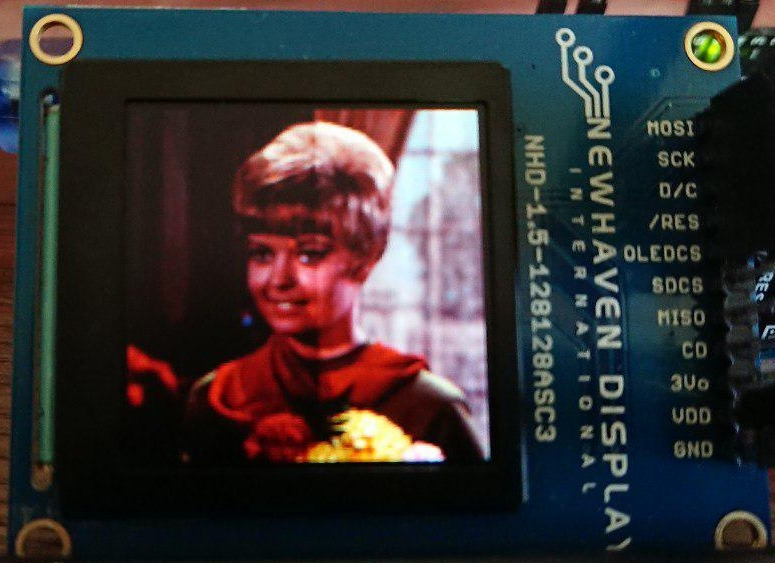
\includegraphics[width=0.4 \columnwidth]{./screenshots/OriginalImageArduino}
                \caption{
                        \label{fig:OriginalImageArduino}
                        The OLED display representing the same image color reduced by \texttt{MATLAB} on the left side of the screen and in its original form on the right side of the screen. The image was loaded in around 20-30 seconds.
                }
            \end{figure}

        \subsubsection{Image Manipulation}
            As a final request of this second laboratory we were asked to implement some image manipulations on the \emph{Arduino} side, in order to analyze possible image distortions different than the ones obtained by running the same manipulations on \texttt{MATLAB}. 
            
            Since the Bytes sent to \emph{Arduino} on the serial port cannot be stored in RAM because if its limited capacity, it is necessary to modify the single Bytes \emph{on-the-fly} just after reception and before sending them again to the display controller.

            To do that we added a piece of code, protected by the pre-processor directive \texttt{IMG\_EDIT} in order to mask or unmask the code prior compilation. 
            We decided to opt for a color manipulation technique, similar to the first manipulation technique we mentioned for the first part of the report. Also in this case, we defined a constant called \texttt{COLOR\_REDUCTION\_PERC} representing the percentage of reduction we want to apply to each channel of the image.

            Since the color reduction must be applied \emph{on-the-fly}, the computation is done in the \texttt{serialEvent()} routine, enclosed between an \texttt{\#if IMG\_EDIT} pre-processor statement: here the reduction value is subtracted to the original value and the new color reduced \texttt{data} variable is sent to the display controller as we said in the previous section. In the following picture (\ref{fig:ColorReductionComparison}) we reported a photo of the OLED display showing a comparison between the same image color reduced by \texttt{MATLAB} (on the right side of the screen) and color reduced \emph{on-the-fly} by \emph{Arduino} (on the left side of the screen).
            From this image it is possible to notice the clear distortion caused by the color reduction applied at run-time to the original image, making such technique not feasible for everyday operations.

            \begin{figure}[htp]
                \centering
                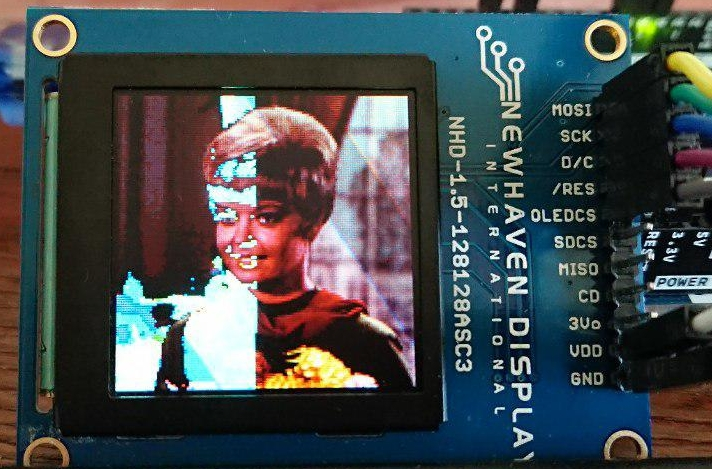
\includegraphics[width=0.4 \columnwidth]{./screenshots/ColorReductionComparison}
                \caption{
                        \label{fig:ColorReductionComparison}
                        The OLED display representing the same image with the two different color reductions applied: on the left the color reduction done by \emph{Arduino}, on the right the color reduction done by \text{MATLAB}.
                }
            \end{figure}


    \subsection{Final Comments}

\end{document}